% --
% theory

\section{Theory}\label{sec:nn_theory}
This section provide the preliminaries to understand the used neural network architectures and the training procedure in general.


% activation functions
\subsection{Activation Functions}\label{sec:nn_theory_acti}
Activation functions for neural networks are non-linear functions that map the sum of the weighted inputs to an output value of a node:
\begin{equation}\label{eq:nn_theory_acti}
  z = h(w \, x^T)
\end{equation}
where $h$ is the activation function, $w \in \R^n$ is an weight vector and $x \in \R^n$ an input vector for one specific node.
One constraint of an activation function is, that an easy computable derivative of this function exist, such that the backpropagation of gradients work.


% cnn
\subsection{Convolutional Neural Networks}\label{sec:nn_theory_cnn}
Covolutional Neural Networks (CNN) as already discussed in \rsec{prev_nn_cnn} use convolutional filters on spatial sections of the input.
Those convolutional filters are also called kernels, for images illustrated as rectangle in 2D space with kernel width $k_w$ and height $k_h$.

The kernel is shifted over its input map in each axis with an operation called \emph{stride}, denoted as $s$, and produce a output map.
The output dimension $o_d$ for striding in along its axis with $s_d$ and kernel size for that axis $k_d$ over the input dimension $i_d$ can be computed as:
\begin{equation}\label{eq:nn_theory_cnn_}
  o_d = \floor*{\frac{i_d + p_d - k_d}{s_d} + 1}
\end{equation}
where $p_d$ is additionally a \emph{padding} term, where for instance for in zero-padding, zeros are added on both sides of the input dimension.
For example if a $16 \times 16$ image is convoluted by a $5 \times 5$ kernel with stride $1$ in each direction and no padding, the output image is $12 \times 12$.
The padding operation has usually the purpose to keep a the output and input dimension the same.
This is used for instance in residual neural networks, where the input to convolutional layers of a block, is bypassed and added to the output of this block again.
Being able to compute the addition operation from input and output of the residual block, their dimensions must be the same.
However in most usual convolutional network applications without residual blocks, it is preferred not to pad the image, so that dimensions are reduced hence parameters and multiplications saved.
Further there exist special convolutional layers that should reduce the dimensions, such as a Max-Pooling layers. 

As already mentioned above CNNs are defined with the amount of input and output channels (feature maps), the kernel size, the stride of the kernel and some other specialties like dilation.
However it is not immediately clear from those parameter, how many convolutional filters are applied and what how the output feature maps are calculated.
Usually in most applications, the convolution to output feature maps are done with:
A typical example is shown in...

\begin{figure}[!ht]
  \centering
    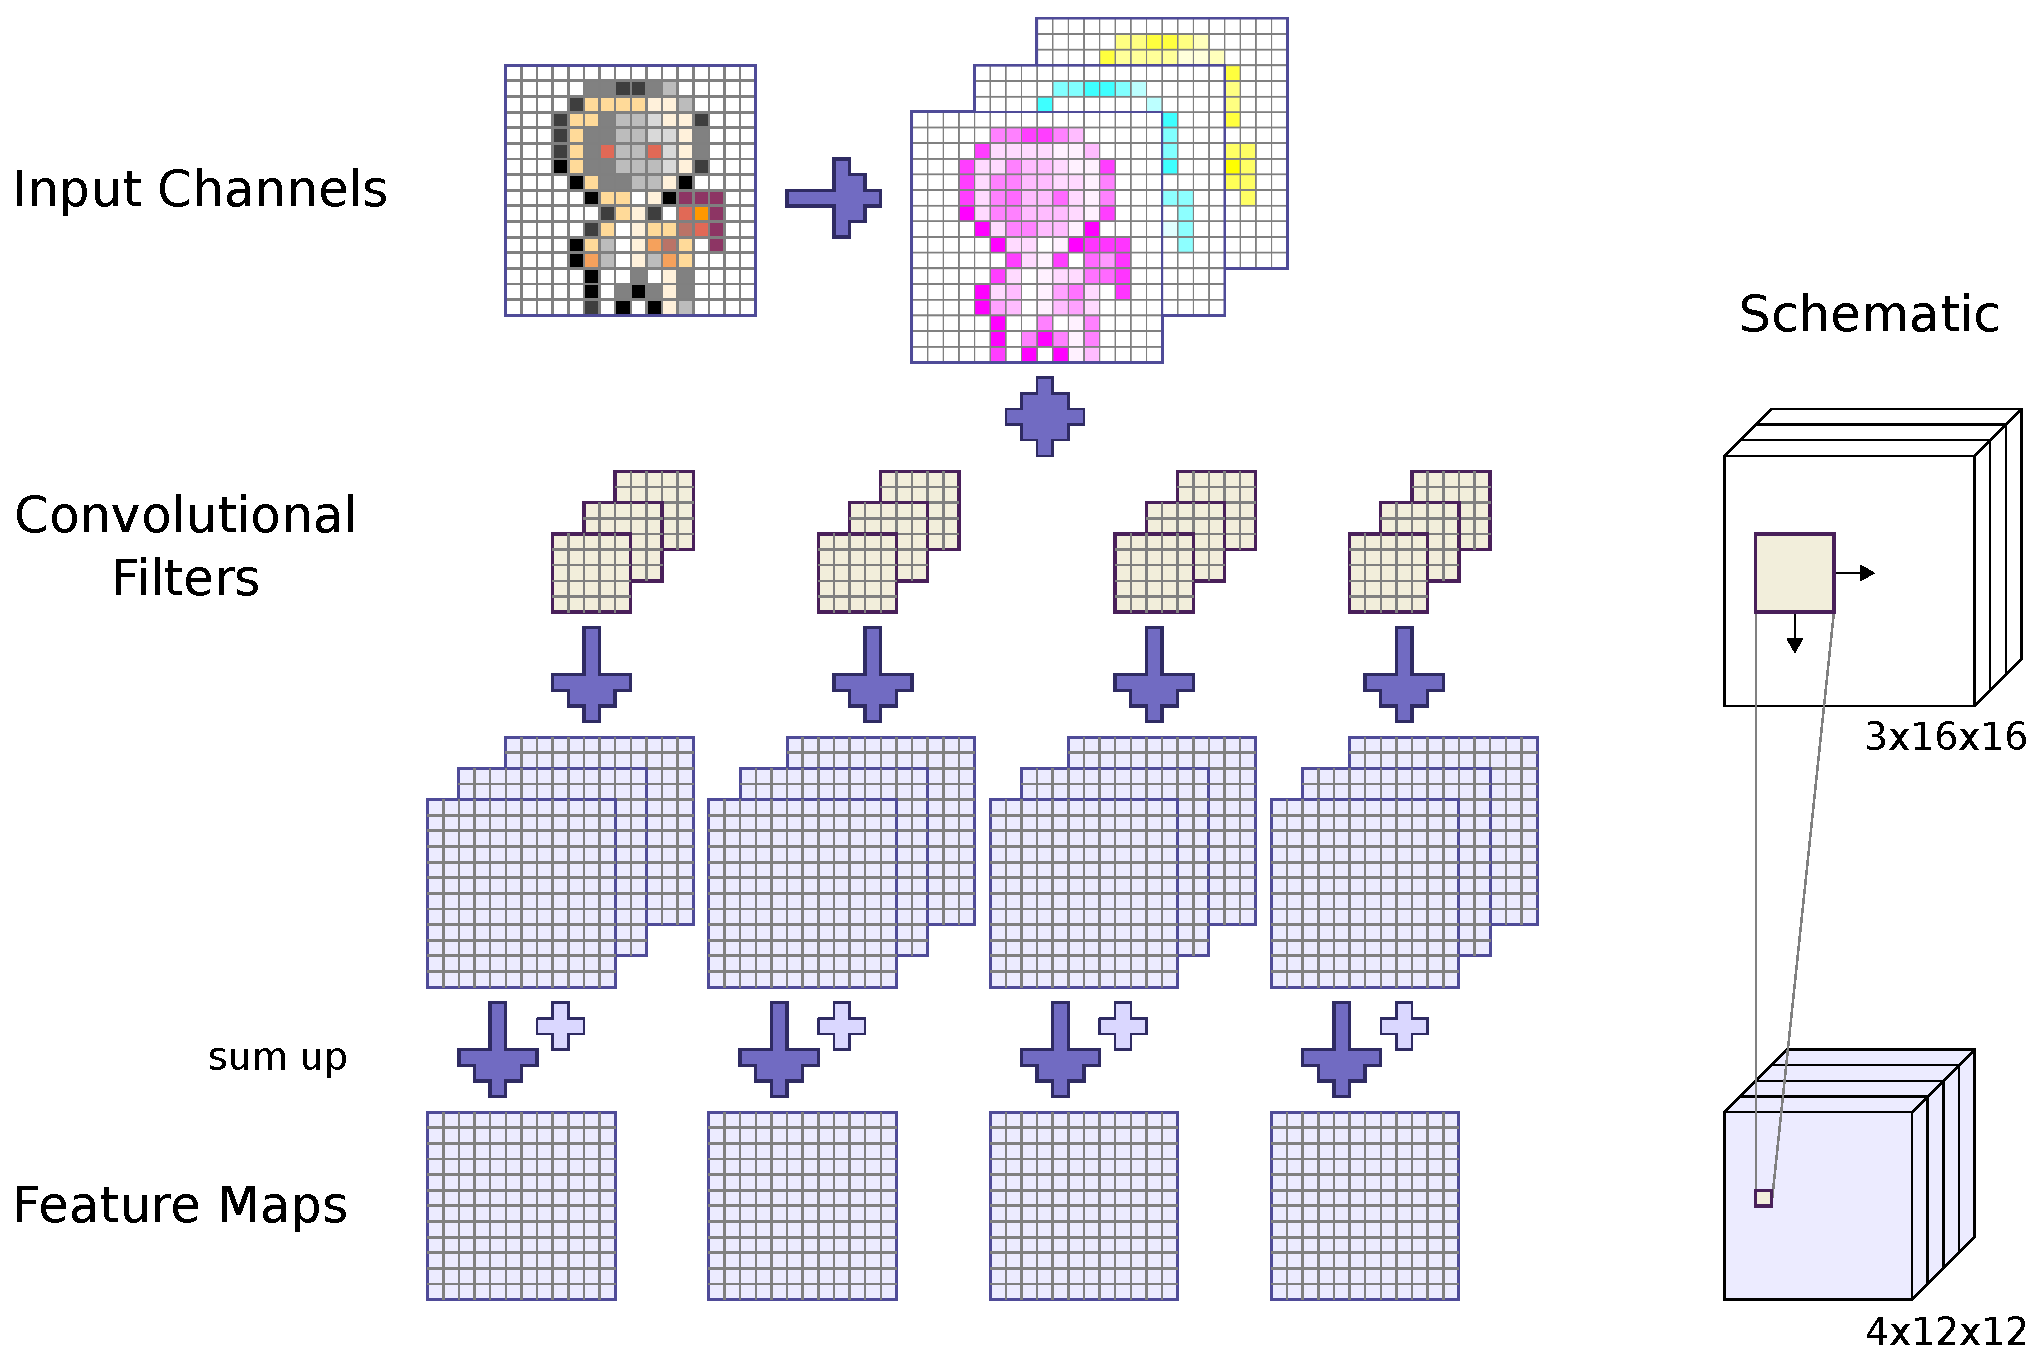
\includegraphics[width=0.6\textwidth]{./4_nn/figs/cnn_basics.eps}
  \caption{CNN basic architecture}
  \label{fig:nn_theory_cnn_basics}
\end{figure}
\FloatBarrier
\noindent

% \begin{figure}[h]
%   \centering{
%   \resizebox{0.5\textwidth}{!}{\input{./4_nn/figs/cnn_basics.tex}}}
%   \caption{CNN basic architecture}
%   \label{fig:nn_theory_cnn_basic}
% \end{figure}
% \FloatBarrier
% \noindent
